\section{Methodology}
%
In this work, we propose \textbf{\method}, a real-time and interactive framework that enables human-garment customization in autoregressive video generation.
% 
Given a reference image $I^{\text{src}}$ and a sequence of $N$ garment images $\langle I^{\text{gar}_1}, \ldots, I^{\textit{gar}_N} \rangle$, our goal is to generate videos in a streaming manner, where each garment is applied to the character at different moments while ensuring coherent human motion.
% 
In Sec.\,\ref{sec:3-1}, we first train a \textbf{Teacher Model with In-Context Learning} conditioned on a reference image and a single garment image.
% 
In Sec.\,\ref{sec:3-2}, we introduce \textbf{Streaming Distillation with In-Context Learning}, featuring an \textit{in-context teacher forcing mask} technique for stable training and a \textit{gradient-reweighted distribution matching distillation} strategy to improve extrapolation consistency.
% 
In Sec.\,~\ref{sec:3-3}, we propose \textbf{Training-Free KV Cache Rescheduling}, which consists of \textit{garment KV refresh}, \textit{historical KV withdraw}, and \textit{reference KV disentangle}, enabling seamless garment switching while maintaining motion coherence.
%
In Sec.\,\ref{sec:3-4}, we develop a \textbf{High-Quality Data Curation Pipeline} to further support training.
% 
The overall pipeline of \method is shown in Figure~\ref{fig:overall_pipeline}.



\begin{figure}[t]
    \centering
    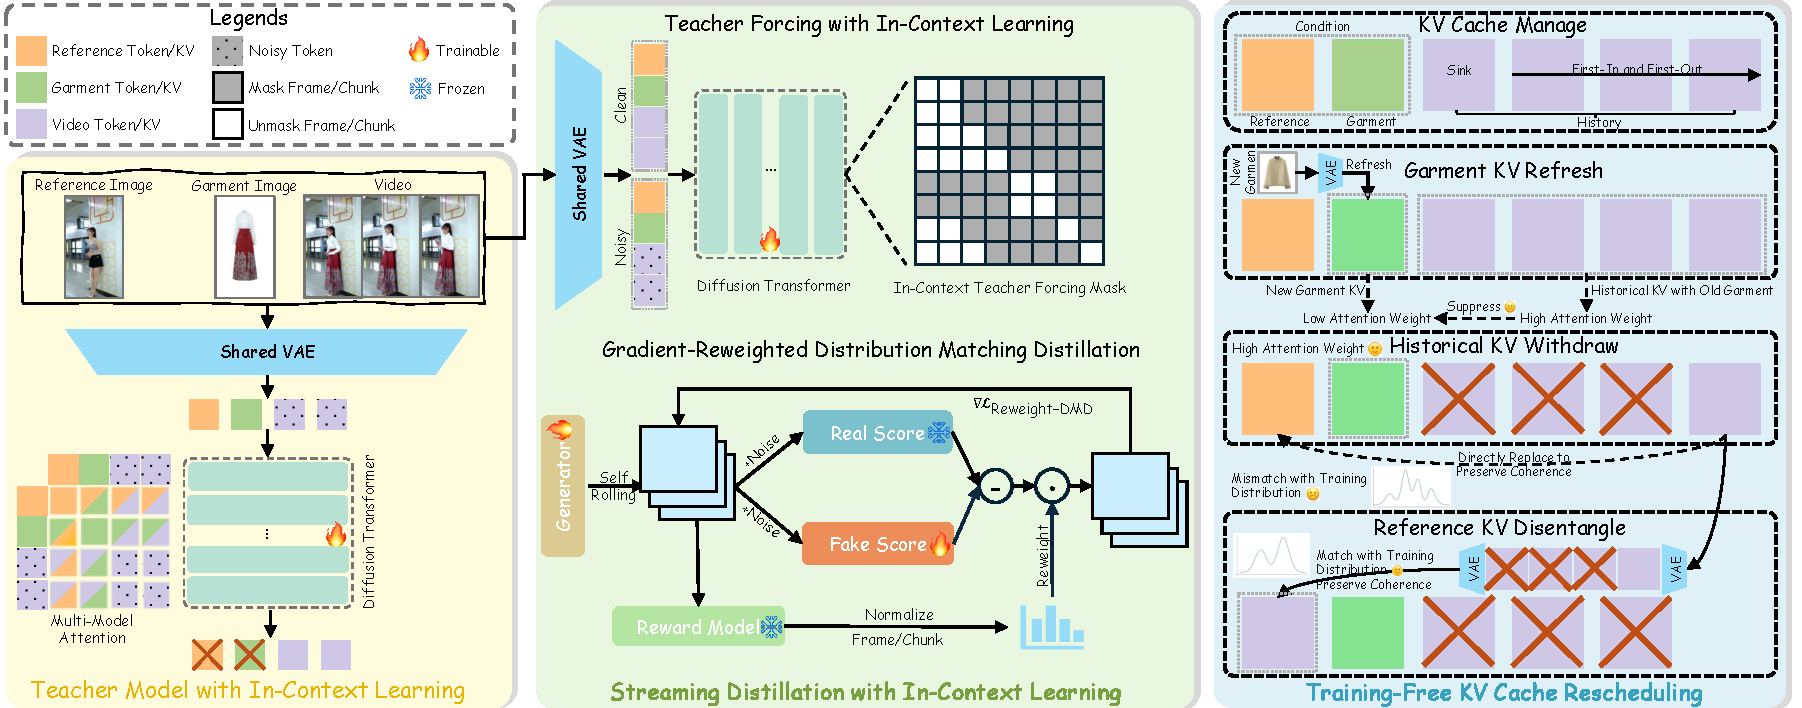
\includegraphics[width=0.98\linewidth]{figures/overall_pipeline.pdf}
    \caption{
    Overall pipeline of \method: \textit{Teacher Model with In-Context Learning}, \textit{Streaming Distillation with In-Context Learning}, and \textit{Training-Free KV Cache Rescheduling}.
    }
    \label{fig:overall_pipeline}
    \vspace{-1.0em}
\end{figure}





\subsection{Teacher Model with In-Context Learning}
\label{sec:3-1}
% 
To enable real-time and interactive human-garment video customization, we first train a bidirectional teacher model conditioned on a reference image and a single garment image.
% 
Unlike prior works~\cite{huang2025live,zhuang2025flashvsr,shin2025motionstream} that rely on auxiliary encoders to process continuous signals, we adopt in-context learning within a unified backbone network to process discrete reference and garment images, eliminating the auxiliary encoders.
% 
\textbf{Notably}, we retain the \textit{image-to-video (I2V) training property}, such that the first generated frame stays consistent with the reference frame, except for the garment information.
\textbf{Meanwhile}, we ensure that \textit{the garment worn by the reference person differs from the target garment}.
This implicitly enables the model to learn single-garment switching while maintaining coherence.

\noindent
\textbf{Shared Latent Space with Varying Noise Levels.}
% 
During training process, a given video $\mathcal{V}$ is encoded into a latent representation $z_{0}^{v}$ by the VAE encoder $\mathcal{E}$.
% 
Instead of introducing an additional encoder, we reuse $\mathcal{E}$ to separately encode the reference image $I^{\text{src}}$ and the garment image $I^{\text{gar}}$ into latent representations $z^{\text{src}}_{0}$ and $z^{\text{gar}}_{0}$.
% 
The whole process can be formulated as follows:
% 
\begin{equation}
    z^{v}_{0} = \mathcal{E}(\mathcal{V});\quad
    z^{\text{src}}_{0} = \mathcal{E}(I^{\text{src}});\quad
    z^{\text{gar}}_{0} = \mathcal{E}(I^{\text{gar}}).
\end{equation}
% 
In this way, all latents can share semantic space without introducing additional parameters.
% 
Subsequently, the video latent $z_{0}^{v}$ is noised according to the flow-matching defined in Eq.\,\ref{eq:1}, while the reference latent $z^{\text{src}}_{0}$ and garment latent $z^{\text{gar}}_{0}$ remain noise-free as conditional inputs.



\noindent
\textbf{Multi-Modal Attention.}
% 
To enable multi-modal interaction within a single backbone, the clean reference latent $\mathbf{z}^{\text{src}}_{0}$, clean garment latent $\mathbf{z}^{\text{gar}}_{0}$, and noisy video latent $\mathbf{z}^{v}_{t}$ are concatenated along the token dimension. The resulting sequence $z_t^{\text{uni}}$ is then projected via learnable matrices $W_q$, $W_k$, and $W_v$, followed by multi-modal attention interaction. The attention output $\mathcal{O}$ can be formulated by:
% 
\begin{equation}
    \mathcal{O} = \text{Softmax}(\frac{(\mathcal{W}_q \cdot z_t^{\text{uni}} )(\mathcal{W}_k \cdot z_t^{\text{uni}})^\top}{\sqrt{d_k}})(\mathcal{W}_v \cdot z_t^{\text{uni}}),
\end{equation}
% 
where $d_k$ denotes the feature dimension.
% 
These shared projection matrices enables global interaction between conditional and video latents without introducing additional parameters.
% 
Finally, the model output retains only the video latent, discarding the reference latent and garment latent.





\subsection{Streaming Distillation with In-Context Learning}
\label{sec:3-2}
%
In this section, we distill the pretrained teacher into a few-step autoregressive student for streaming generation.
% 
Prior works~\cite{yin2025slow,huang2025self,zhu2026causal} show that direct distillation is challenging and adopt a two-stage strategy comprising ODE initialization and distribution matching distillation~\cite{yin2024improved}.
% 
To better adapt to our setting, we instead adopt \textit{teacher forcing}~\cite{gao2024ca2,hu2024acdit,zhang2025test} to initialize the student model, followed by \textit{gradient-reweighted distribution matching distillation} to improve extrapolation consistency.



\noindent
\textbf{In-Context Teacher Forcing Mask.}
% 
The teacher forcing fine-tunes the pretrained multi-step bidirectional model into a multi-step autoregressive model using clean data.
% 
However, unlike prior approaches~\cite{huang2025live,zhuang2025flashvsr,shin2025motionstream} that inject control signals via adapters, our model incorporates these signals through in-context token concatenation, making standard teacher forcing inapplicable.
To address this, we design an in-context teacher forcing mask for training, with the toy examples shown in Figure~\ref{fig:overall_pipeline}.
% 
Specifically, in addition to the noisy sequence $\langle z^{\text{src}}_0, z^{\text{tar}}_0, z^{v}_t \rangle$, we symmetrically concatenate its clean counterpart $\langle z^{\text{src}}_0, z^{\text{tar}}_0, z^{v}_0 \rangle$ and feed the resulting sequence into the model.
% 
For the conditioning signals $z^{\text{src}}_0$ and $z^{\text{tar}}_0$, we apply a dedicated masking strategy such that all generated frames can attend to them, while $z^{\text{src}}_0$ and $z^{\text{tar}}_0$ cannot access any future generated frames.
% 
In this way, when predicting the next frame (chunk), model conditions on ground-truth historical frames and conditional signals.



\noindent
\textbf{Gradient-Reweighted Distribution Matching Distillation.}
% 
Based on the autoregressive model fine-tuned with teacher forcing, we further apply distribution matching distillation (DMD) for few-step generation and combine it with Self-Forcing~\cite{huang2025self} to better align training with inference.
%
However, we observe that directly applying DMD often leads to distorted human motions during extrapolation.
%
We attribute this to the unequal difficulty of frames in self-rolling generation: errors accumulate over time, making later frames more prone to drift, whereas vanilla DMD weights all frames equally.
%
To resolve this, we propose an adaptive gradient reweighting strategy that increases the weights of low-quality frames while decreasing those of high-quality ones during distillation.
% 
Specifically, we use an aesthetic reward model $\mathcal{R}$ to estimate frame quality during distillation and normalize the resulting scores into frame-wise gradient weights.
% 
In this way, the Eq.\,\ref{eq:3} can be rewritten as:
% 
\begin{equation}
\begin{gathered}
\nabla \mathcal{L}_{\text{Reweight-DMD}} 
= - \mathbb{E}_{t} \Biggl[
\int 
\mathcal{A}^{1:f} (G(\epsilon)) 
\cdot
\big(
s_{\text{real}}^{1:f} (\phi(G(\epsilon), t), t)
-
s_{\text{fake}}^{1:f} (\phi(G(\epsilon), t), t)
\big)
\cdot
\frac{d G_{\theta}(\epsilon)}{d\theta}
\cdot
d\epsilon
\Biggr], \\
\mathcal{A}^{i} (G(\epsilon)) = \frac{\exp(-\mathcal{R} (G^{i}(\epsilon)) / \tau)}{\sum_{j=1}^{f} \exp(-\mathcal{R} (G^{j}(\epsilon)) / \tau)}, \quad i=1, \dots, f,
\end{gathered}
\end{equation}
% 
where $\tau$ denotes the temperature coefficient that controls the relative weight. Note that this approach is not restricted to aesthetic rewards and can naturally accommodate other reward models.







\subsection{Training-Free KV Cache Rescheduling}
\label{sec:3-3}
%
Given the distilled few-step autoregressive models, we manage KV cache to enable stable long-video extrapolation.
%
In detail, the reference KV entry $KV^{\text{src}}$ and garment KV entry $KV^{\text{gar}}$ are persistently stored in the KV cache as conditioning signals.
% 
Following prior work~\cite{yang2025longlive,yesiltepe2025infinity}, we also retain the KV entries of the initial frame (chunk), $KV^{0}$, as an attention sink to improve stability during extrapolation.
% 
All remaining KV entries follow a first-in and first-out policy when the cache exceeds its maximum size.
% 
Formally, at the generation of $\text{k-th}$ frame, the KV cache is defined as:
% 
\begin{equation}
    \text{KV Cache} \, := \, \langle KV^{\text{src}}, KV^{\text{gar}}, KV^{0}, KV^{\text{Max(1, k - M + 4)}}, \dots, KV^{\text{k}} \rangle,
\end{equation}
% 
where $M$ is the maximum KV cache size.
%
To enable \textbf{interactive multi-garment switching while maintaining coherence}, we reschedule the KV cache via three mechanisms: \textit{Garment KV Refresh}, \textit{Historical KV Withdraw}, and \textit{Reference KV Disentangle}, as illustrated in Figure~\ref{fig:overall_pipeline} (right).


\begin{figure}[t]
    \centering
    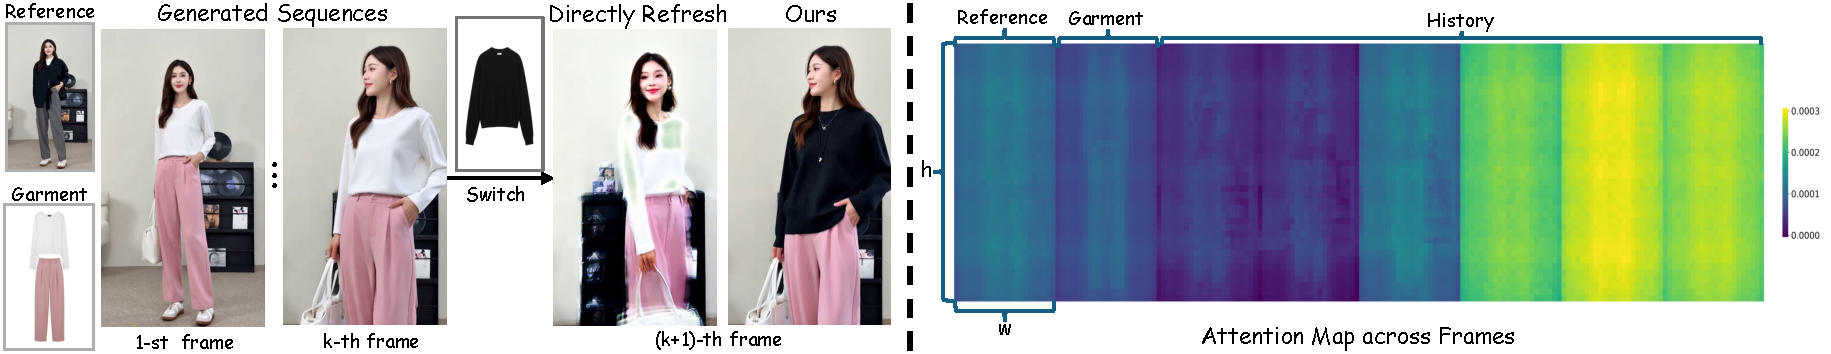
\includegraphics[width=0.98\linewidth]{figures/analysis.pdf}
    \caption{
    (Left) Generated sequences during garment switching. Directly refreshing the garment KV fails to change the subject’s clothing, while our KV cache rescheduling enables garment-switching and motion coherence.
    % 
    (Right) Average attention visualization of newly generated frames over historical and conditional KV. The model attends more to historical KV than to conditional KV.
    }
    \label{fig:analysis}
    \vspace{-1.0em}
\end{figure}


\noindent
\textbf{Garment KV Refresh.}
% 
To switch the character with a new garment $I^{\text{gar}_2}$ during generation, we refresh the garment KV in the cache.
Specifically, $I^{\text{gar}_2}$ is encoded into $z^{\text{gar}_2}$ by VAE, and the corresponding  $KV^{\text{gar}_{2}}$ are obtained via a forward pass. 
We then replace the old $KV^{\text{gar}}$ in the cache with new new $KV^{\text{gar}_{2}}$, so that subsequent frames are generated conditioned on the updated garment.



\noindent
\textbf{Historical KV Withdraw.}
% 
However, as shown in Figure~\ref{fig:analysis} (left), directly refreshing garment KV is insufficient to change the garment in subsequent generated frames.
%
To analyze this phenomenon, we visualize the average attention weights of newly generated latents over conditional and historical KV. In Figure~\ref{fig:analysis} (right), attention is more concentrated on historical KV rather than conditional KV.
This indicates that, under streaming eneration with in-context learning, the model relies more on historical context than on conditional signals.
Consequently, the old garment from historical frames tends to persist in newly generated frames, rendering the new garment signal ineffective.
%
Therefore, we withdraw the historical KV, encouraging the model to focus on the new garment KV.



\noindent
\textbf{Reference KV Disentangle.}
%
While withdrawing historical KV enables garment switching, it weakens temporal coherence across the switching frame.
% 
Recall that we deliberately \textbf{I2V property} during pre-training, in which the first generated frame remains consistent with the reference frame except for garment information. This endows the model with an implicit capability to maintain temporal coherence during single-garment switching.
% 
To enable multi-garment switching during generation, the key is to \textit{align the distribution of the new conditioning signal with that of the original conditioning signal}.
% 
To this end, we replace old $KV^{\text{src}}$ with the $KV^{\text{k}}$ extracted from the last historical frame.
% 
\textbf{Notably}, the new reference KV corresponds to four decoded frames, mismatching with the old reference KV that corresponds to single-frame.
We thus perform a VAE decode-encode process to disentangle the last decoded frame, followed by an additional forward to obtain new reference KV.





\subsection{High-Quality Data Curation Pipeline}
\label{sec:3-4}
%
To further support teacher model pre-training and streaming distillation post-training, we design a data curation pipeline to construct samples of the reference image $I^{\text{src}}$, garment image $I^{\text{gar}}$, video sequence $\mathcal{V}$ and corresponding prompt.
The pipeline consists of four stages: \textit{1. General Coarse-to-Fine Video Filtering}, \textit{2. Static-Dynamic Video Captioning}, \textit{3. Fine-Grained Garment Images Extraction}, and \textit{4. Adaptive Reference Images Construction}.
We provide implementation details in the \textbf{Appendix}.
